% article example for classicthesis.sty
\documentclass[10pt,a4paper]{article} % KOMA-Script article scrartcl
\usepackage{import}
\usepackage{xifthen}
\usepackage{pdfpages}
\usepackage{transparent}
\newcommand{\incfig}[1]{%
    \def\svgwidth{\columnwidth}
    \import{./figures/}{#1.pdf_tex}
}
\usepackage{lipsum}     %lorem ipsum text
\usepackage{titlesec}   %Section settings
\usepackage{titling}    %Title settings
\usepackage[margin=10em]{geometry}  %Adjusting margins
\usepackage{setspace}
\usepackage{listings}
\usepackage{amsmath}    %Display equations options
\usepackage{amssymb}    %More symbols
\usepackage{xcolor}     %Color settings
\usepackage{pagecolor}
\usepackage{mdframed}
\usepackage[spanish]{babel}
\usepackage[utf8]{inputenc}
\usepackage{longtable}
\usepackage{multicol}
\usepackage{graphicx}
\graphicspath{ {./Images/} }
\setlength{\columnsep}{1cm}

% ====| color de la pagina y del fondo |==== %
\pagecolor{white}
\color{black}



\begin{document}
    %========================{TITLE}====================%
    \title{\rmfamily\normalfont\spacedallcaps{ Taller 1 de Teoría de Grafos }}
    \author{\spacedlowsmallcaps{Rodrigo Castillo}}
    \date{\today}

    \maketitle


     % ====| Loguito |==== %
    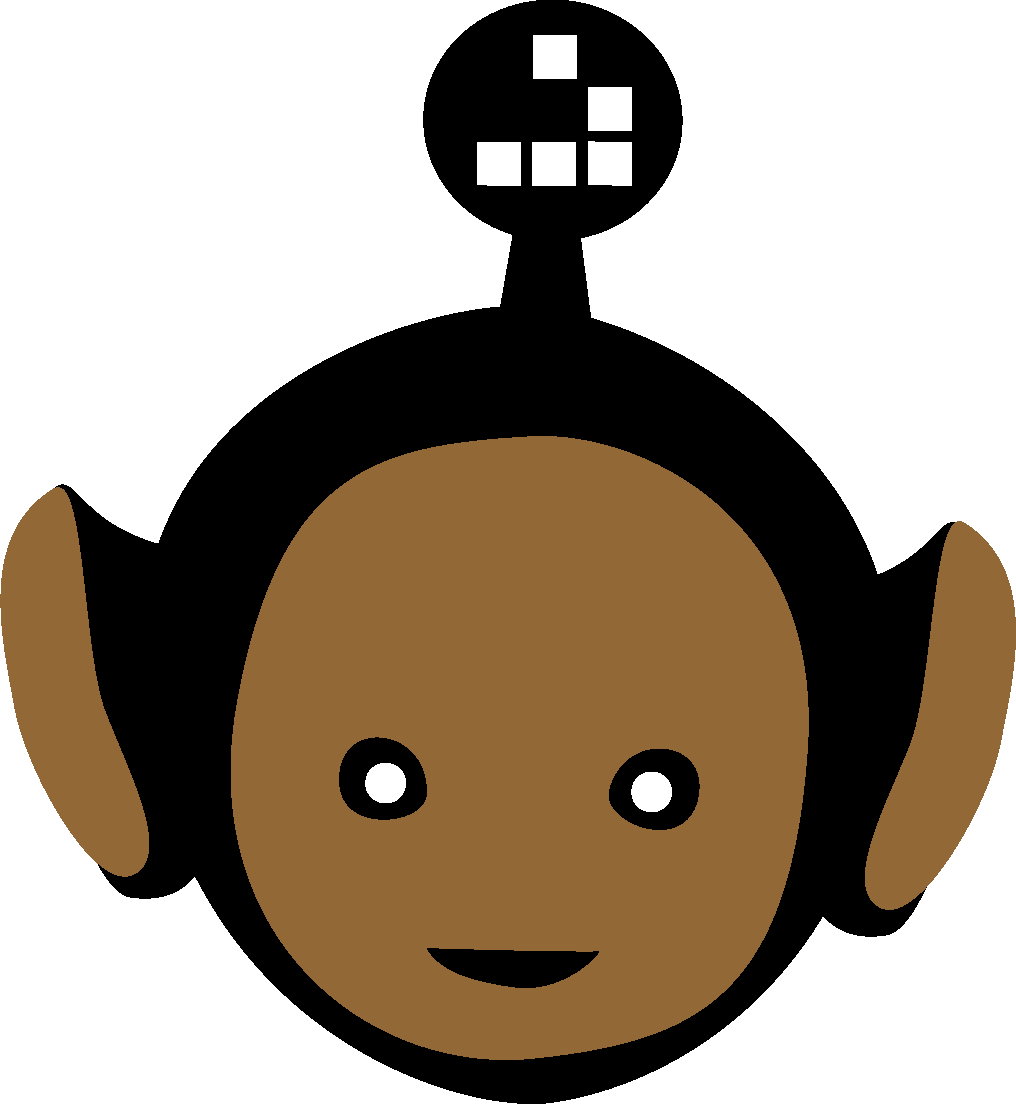
\includegraphics[width=0.1\linewidth]{negro_cara.png}
    %=======================NOTES GOES HERE===================%
    \section{Determine si las siguientes parejas de grafos son isomorfas.
    Defina el isomorfismo o use invariantes para probar que no son isomorfas}
        \subsection{Pareja 1:}
            \begin{figure}[h]
                \centering
                \incfig{grafouno}
                \caption{grafouno}
                \label{fig:grafouno}
            \end{figure}

            estos grafos si son isomorfos, usaré el siguiente dibujo para
            exponer la biyección:

            \begin{figure}[h]
                \centering
                \incfig{biyecuno}
                \caption{biyecuno}
                \label{fig:biyeccion 1}
            \end{figure}

        \subsection{Pareja 2:}
            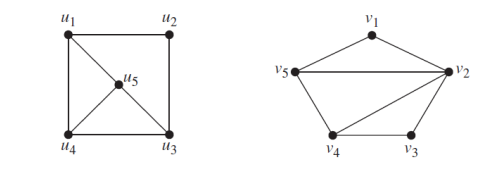
\includegraphics[width=0.5\linewidth]{parej2.png}
            \\
            \color{teal}
            no son isomorfos, esto para porque el maximo grado de una arista en
            el grafo de la izquierda es de 4 y en el de la derecha es de 3, el
            maximo grado de una arista es un invariante.
            \color{black}

        \subsection{Pareja 3:}
            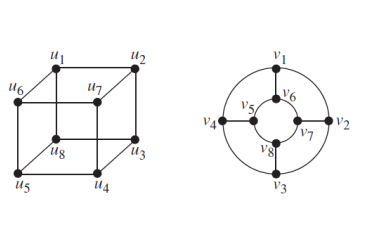
\includegraphics[width=0.8\linewidth]{pareja3.png}
            \\
            % ====| ISOMORFISMO ACA |==== %
            \\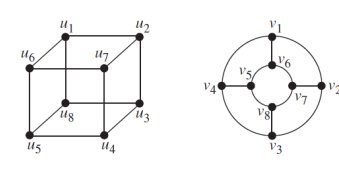
\includegraphics[width=0.8\linewidth]{grafotres.png}
            \\
            isomorfismo : \\
            $ u1 \implies v1  $
            \\ $ u2 \implies v2  $
            \\ $ u6 \implies v4  $
            \\ $ u7 \implies v3  $
            \\ $ u4 \implies v5  $
            \\ $ u3 \implies v6  $
            \\ $ u5 \implies v7  $
            \\ $ u8 \implies v8  $

    \section{construya la matriz de adyacencia $ A  $ del siguiente grafo:}
        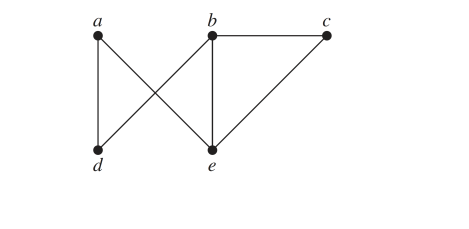
\includegraphics[width=0.8\linewidth]{grafoadj.png}
        \\
        \subsection{Matriz de adyacencia}
            \begin{pmatrix}
                  0 & 0 & 0 & 1 & 1
                \\0 & 0 & 1 & 1 & 1
                \\0 & 1 & 0 & 0 & 1
                \\1 & 1 & 0 & 0 & 0
                \\1 & 1 & 1 & 0 & 0
            \end{pmatrix}
            \subsubsection{calcule $ A ^{2}   $ }
                % ====| PREGUNTAR ESTO BIEN PORQUE ESTÁ UN POCO CHISTOSO |==== %
                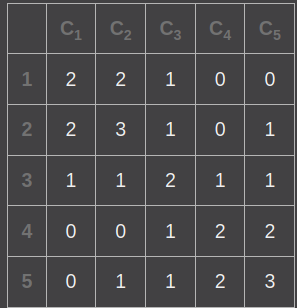
\includegraphics[width=0.8\linewidth]{multiplicacion.png}
                \\ (esta propiedad me parece especialmente poderosa :O)

            \subsubsection{escriba una $ b-c  $ caminata con longitud 2, y 3 $
            e-e  $ caminatas de longitud 2}
                $ b-c  $ caminata de longitud 2

                caminata:
                \begin{equation}
                    [b-e , c-e]
                \end{equation}
                3 caminatas $ e-e  $ de longitud 2
                \begin{equation}
                    [e-b , b-e] , [e-a,a-b] , [e-c,c-e]
                \end{equation}

            \subsubsection{calcule $ A ^{3}   $ }
            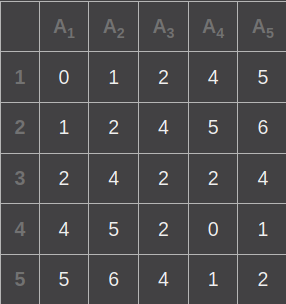
\includegraphics[width=0.8\linewidth]{alatres.png}
            \\

            \subsection{Escriba cinco $ a-e  $ -caminatas de longitud 3 y
            verifique que no existen $ d-d  $ caminatas de longitud 3}
                $ a-e  $ caminatas de longitud 3 :
                \begin{equation}
                    [a-d , d-b , b-e] , [a-e , e-c , c-e] , [a-e,e-a,a-e] , [a-e, e-b , b-e] , [a-d , d-a , a-c]
                \end{equation}

            no existen caminatas de longitud 3:
            \\note que el siguiente grafo es isomorfo al grafo dado.
                % ====| DIBUJO |==== %
            \begin{figure}[h]
                \centering
                \incfig{camimatastres}
                \caption{camimatastres}
                \label{fig:camimatastres}
            \end{figure}
            \\en este grafo se puede ver que no existen d-d caminatas de
            longitud 3, sin embargo, es trivial verlo en los resultados de $ A
            ^{3}   $ pues sabemos que $ A ^{3}   $ nos devuelve la cantidad de
            caminatas que hay de un vértice a otro.

            \subsubsection{Formule una proposición que resuma los resultados
            observados en los ejercicios anteriores.}
                $ A ^{n}   $ nos retorna la cantidad de $ n-caminatas  $ que
                hay de un vértice a otro y ésto es muy poderoso.



    \section{Pruebe que un grafo es conexo si y solo si para toda partición de
    sus vértices en dos subconjuntos no-vacı́os hay al menos una arista con
    puntos finales en ambos conjuntos}
        $ \implies  $
        \\ suponga que K es un grafo conexo, luego para cualquier par de
        vértices $ a,b \in K  $  se tiene que existe una $ a,b-caminata  $ y
        suponga además que existe una partición de vértices en dos subconjuntos
        no vacíos de $ K  $ tales que no existe una arista con puntos finales
        en ambos conjuntos, luego existen dos vértices $ a,b  $ tales que no
        existe una $ a,b-caminata $ , por lo tanto $ K  $ es un grafo disconexo
        .
        \\ $ \impliedby  $
        \\ suponga que $ K  $ es un grafo para el cuál conjuntos no vacios,
        existe una arista con puntos finales en ambos conjuntos , sean $ a,b  $
        vértices de $ K  $ , suponga que $ a \in P  $ y que $ b \in O  $ siendo
        $ O,P  $ subconjuntos no vacios de $ K  $ , por lo tanto, existe una
        arista que une a $ P-K  $ , luego existe una caminata $ a,b  $ , por lo
        tanto, para cualquier par de vértices $ a,b \in K$ se tiene que existe
        una $ a-b  $ caminata, por lo tanto, existe un $ a-b   $ camino, luego
        $ K  $ es conexo.

    \section{escriba (si es posible) un circuito o sendero euleriano en el
    siguiente grafo}
    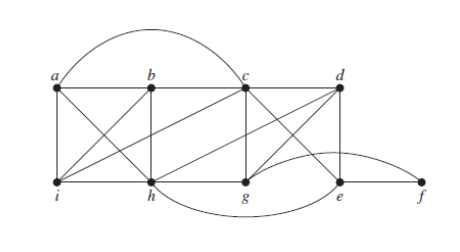
\includegraphics[width=0.8\linewidth]{grafofinal.png}
    si existe un circuito euleriano en el grafo , pues sus aristas son pares.




















    %=======================NOTES ENDS HERE===================%

    % bib stuff
    \nocite{*}
    \addtocontents{toc}{\protect\vspace{\beforebibskip}}
    \addcontentsline{toc}{section}{\refname}
    \bibliographystyle{plain}
    \bibliography{../Bibliography}
\end{document}
